\section{Annual Execution and Human Escalation}
\subsection{Candidate trades and the cost gate}
At each annual review, the advisor checks for escalation before considering a trade. Let $p$ denote current portfolio weights and $w^*$ the frozen strategic anchor for the investment horizon. The five candidates are
\begin{equation}
w_\lambda=p+\lambda(w^*-p),\qquad
\lambda\in\{0,.25,.50,.75,1\}.
\end{equation}
Here, $\lambda=0$ keeps holdings and $\lambda=1$ restores the anchor. Training returns supply the mean $\mu$ and regularized covariance $\Sigma=0.75S+0.25\operatorname{diag}(S)+10^{-10}I$. The tracking score and fractional trading cost are
\begin{equation}
A(w)=1+\mu^{\mathsf T}w^*-\frac{\gamma}{2}(w-w^*)^{\mathsf T}\Sigma(w-w^*),
\qquad f_\lambda=\frac{c}{2}\lVert w_\lambda-p\rVert_1.
\end{equation}
The return term is shared across candidates; the quadratic term penalizes departure from the anchor. If any score is nonpositive or nonfinite, the advisor requests human review. Otherwise, it selects $j$ maximizing $(1-f_\lambda)A(w_\lambda)$ and accepts a trade only if
\begin{equation}
\frac{A(w_j)-A(p)}{A(w_j)}>f_j+0.0001.
\label{eq:gate}
\end{equation}
The extra 0.0001 is a one-basis-point safety margin. If the selected candidate fails this strict gate, holdings are kept; lower-ranked candidates are not tried. This score measures tracking benefit, not a guaranteed increase in future wealth.

\subsection{Four observable actions}
Before trading, the advisor compares observed real drawdown with the training-based threshold
\begin{equation}
\tau=\operatorname{clip}\!\left(1.5\,\Pninety(D_{\rm train,annual}),\ 0.10,\ 0.75\right),
\end{equation}
where $D_{\rm train,annual}$ comes from fee-paying annual rebalancing to the same anchor. For 30-year Balanced A, $\tau=\ReviewThreshold\%$. Table~\ref{tab:actions} distinguishes the four actions. Escalation takes priority over candidate selection; while review is pending, the engine holds existing assets and suspends automatic trading.

\begin{table}[h!]
\centering
\caption{Annual action rules. Accepted trades are classified against the previously recorded execution target, not necessarily the strategic anchor.}
\label{tab:actions}
\begin{tabularx}{\linewidth}{lX}\toprule
Action & Decision rule\\\midrule
1. Keep holdings & The selected step is zero or fails Equation~\eqref{eq:gate}; no trade fee is charged.\\
2. Rebalance & The accepted trade restores the recorded execution target.\\
3. Change target & The accepted trade sets a different execution target; $w^*$ remains fixed.\\
4. Request human review & Observed drawdown reaches $\tau$, or a candidate score is invalid; existing assets remain invested.\\
\bottomrule\end{tabularx}
\end{table}

\subsection{Customer-facing explanation}
Every accepted adjustment uses this 20-word explanation, within the required 50-word limit:
\begin{quote}
``This adjustment moves your investments toward the strategic allocation. Its estimated risk-adjusted benefit exceeds trading costs. Investment losses remain possible.''
\end{quote}

\clearpage
\section{Final Evaluation Results}
\subsection{Higher growth comes with greater drawdown}
Table~\ref{tab:performance} compares policies on the same 60 final scenarios, charging 0.25\% of money moved. Equal-weight annual rebalancing is the required baseline; same-anchor annual and hold controls isolate execution effects.

\begin{table}[h!]
\centering
\caption{Thirty-year final outcomes across 60 scenarios (\%). $G$: net real CAGR; $D$: maximum real drawdown. Trade rate excludes initial allocation.}
\label{tab:performance}
\begin{tabular}{lrrrrr}\toprule
Policy & Med. $G$ & P10 $G$ & Med. $D$ & P90 $D$ & Trades\\\midrule
\tableinput{generated/performance.tex}
\bottomrule\end{tabular}
\end{table}

\begin{figure}[h!]
\centering
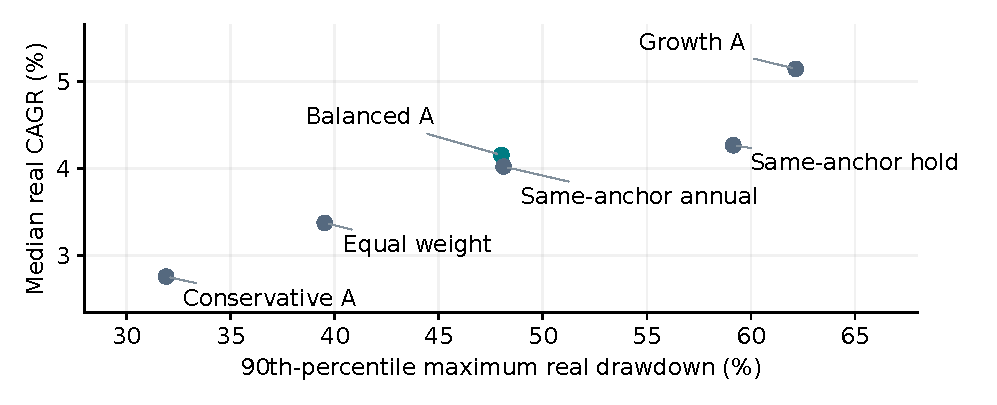
\includegraphics[width=\linewidth]{figures/risk_growth.pdf}
\caption{Thirty-year median growth versus P90 drawdown across 60 scenarios at the base fee. P90 is not a loss guarantee.}
\label{fig:riskgrowth}
\end{figure}

Balanced A gained \GrowthGain{} percentage points (pp) of median growth over equal weight, with \RiskIncrease{} pp more P90 drawdown (Figure~\ref{fig:riskgrowth}). Its median annual volatility was \BalancedVolatility\%, compared with \EqualVolatility\% for equal weight.

\begin{table}[h!]
\centering
\caption{Paired bootstrap comparisons, Balanced A minus equal weight (pp); 4,000 complete-scenario resamples.}
\label{tab:paired}
\begin{tabular}{lrrr}\toprule
Metric & Difference & 95\% interval & Family-adjusted 95\%\\\midrule
Median $G$ & +\GrowthGain & [\GrowthCILower, \GrowthCIUpper] & [\GrowthCIFamilyLower, \GrowthCIFamilyUpper]\\
P90 $D$ & +\RiskIncrease & [\LossCILower, \LossCIUpper] & [\LossCIFamilyLower, \LossCIFamilyUpper]\\
\bottomrule\end{tabular}
\end{table}

Family adjustment covers 20 nonbaseline policies within each endpoint, horizon, and cost; it does not cover the whole adaptive research process.

Against same-anchor annual rebalancing, Balanced A gained \AnnualGrowthGain{} pp of median growth with nearly unchanged P90 drawdown. Mean real fees fell \CostSaving\%, from \AnnualCost{} to \BalancedCost{}. Its trade rate was \BalancedTrades\% (\IncludingInitialTrades\% including initial allocation). Relative to holding the anchor, P90 drawdown fell \HoldRiskReduction{} pp and median growth fell \HoldGrowthLoss{} pp. These comparisons favour selective rebalancing when fees and tail losses both matter.

\subsection{Customer outcomes at their actual horizons}
Table~\ref{tab:customers} uses each customer's actual horizon and frozen assignment. A and D were referred for human review; dashes indicate no automated investment path. Breaches mean maximum drawdown exceeded the customer's stated tolerance.

\begin{table}[h!]
\centering
\caption{Final customer outcomes (growth and drawdown in \%; 60 scenarios).}
\label{tab:customers}
\begin{tabular}{crrrrrl}\toprule
Customer & $H$ & Med. $G$ & P10 $G$ & Med. $D$ & P90 $D$ & Breaches\\\midrule
\tableinput{generated/customers.tex}
\bottomrule\end{tabular}
\end{table}

\begin{table}[h!]
\centering
\caption{Customer risk and trading. Terminal loss means final real wealth below 100; trade rates exclude initial allocation.}
\label{tab:customerrisk}
\begin{tabular}{crlr}\toprule
Customer & Median volatility (\%) & Terminal losses & Trade rate (\%)\\\midrule
\tableinput{generated/customer_risk.tex}
\bottomrule\end{tabular}
\end{table}

For B, P90 drawdown exceeded the 25\% tolerance, with breaches in 7 of 60 scenarios. Eligibility screens breach probability, rather than imposing a guaranteed loss limit. E's negative P10 growth and 9 terminal losses highlight the risk of its six-year horizon despite positive median growth. B, C, and E requested human review in 2, 3, and 0 scenarios, respectively. All assignments remained unchanged after final evaluation.

\subsection{A severe path exposes the limits of escalation}
In scenario 155, Balanced A peaked at \SeverePeak{} in year 6 and ended at \SevereTerminal{} (Figure~\ref{fig:severe}). Its \SevereLoss\% maximum drawdown and \SevereGrowth\% real CAGR show the limits of annual escalation.

\begin{figure}[h!]
\centering
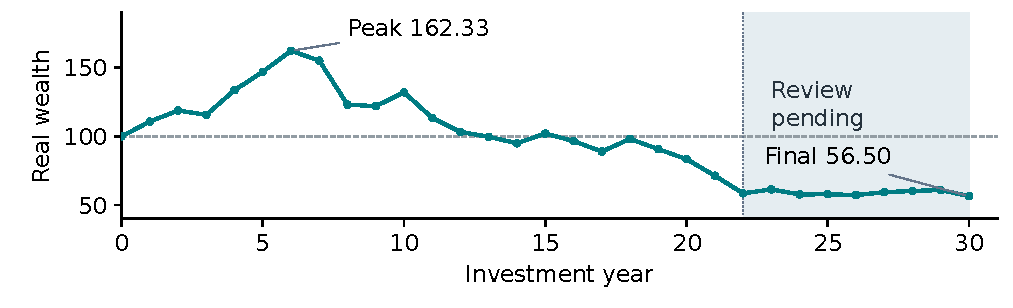
\includegraphics[width=\linewidth]{figures/severe_path.pdf}
\caption{Saved real wealth for scenario 155, starting from 100. Lines join year-end observations; shading marks pending review, beginning before year 23.}
\label{fig:severe}
\end{figure}

Six post-initial trades preceded the review request before the year-23 return. Automatic trading then stopped, but the existing holdings remained exposed. Across all 60 Balanced paths, drawdown CVaR90 was \BalancedTailLoss\%, versus P90 drawdown of \BalancedPninety\%.
